\documentclass[twocolumn,11pt]{article}
\usepackage{savetrees}
% a more conservative option:
% \documentclass[]{article}
% \usepackage{fullpage}

%AMS-TeX packages
\usepackage{amssymb,amsmath,amsthm} 
%geometry (sets margin) and other useful packages
%\usepackage[letterpaper, top=0.75in, left=1.0in, total={6.0in,9in}]{geometry}
\usepackage{graphicx,ctable,booktabs}
\usepackage{enumerate}
\usepackage{float}
\usepackage{wrapfig}
\usepackage{mathrsfs}
%\usepackage{nicefrac}
\usepackage{epsfig}
\usepackage{epstopdf}

% for boxed figs
\usepackage{float}
\floatstyle{boxed} 
\restylefloat{figure}

% for 21 savage
\usepackage{hyperref}

% for degrees
\usepackage{gensymb}

% use color for blue text
\usepackage{color}

% blue text for questions
\newcommand{\bt}[1]{\textcolor{blue}{#1}}

\title{PY 202, 4/10/17}
\author{John M. Lynch\footnote{Undergraduate ECE/Physics, NCSU, Raleigh, NC 27705. E-Mail: \texttt{jmlynch3@ncsu.edu}}}
\date{\today}

\begin{document}
  \maketitle
  
  \section*{Topics for Exam}
  	\begin{enumerate}
  		\item LC Circuits
		\item EM waves
		\item reflection, refraction (31)
		\item polarization (31)
		\item mirrors, lenses (32)
  	\end{enumerate}
	
	\section*{HW 32}
		\begin{enumerate}
			\item only one problem on WebAssign!
			\item downside: quite a bit of ray-tracing on rest of HW (\LaTeX will be difficult)
		\end{enumerate}
	
	\section*{Quiz Review}
		\begin{enumerate}
			\item reflection \& refraction: It's the angles with respect to the \emph{normal} that
				  matter, not the surface!
		\end{enumerate}
	
	\section*{Today's Quiz}
	\begin{enumerate}
		\item If you are looking at a rock on the bottom of a stream, what do you see? Does it seem
			  closer, further away, or at the correct depth?
			  \begin{enumerate}
			  	\item A (correct, 0.35): You think you see it close along your line of sight,
					  but in reality it rests much lower, on the lake floor.
				% IMAGE Q1
				\begin{figure}
					\begin{center}
						\caption{Quiz 1}
						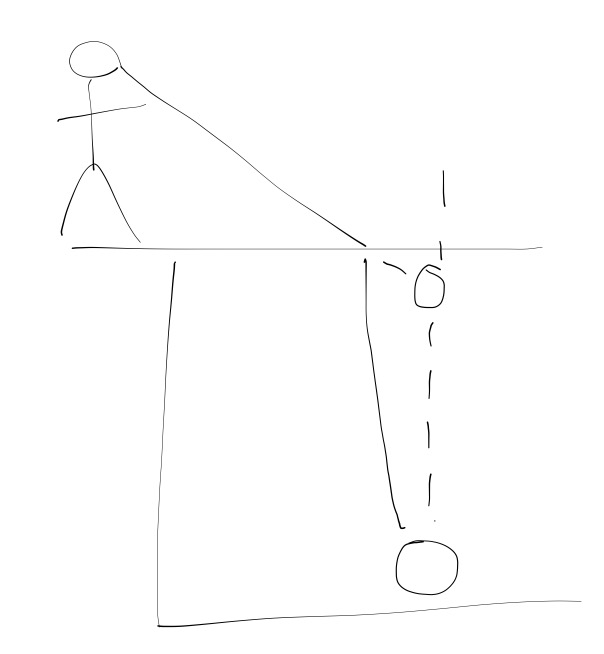
\includegraphics[scale=0.4]{q1.png}
					\end{center}
				\end{figure}
			  \end{enumerate}
		\item light is incident at $55 \degree$ on a water/air interface. Is there reflection (B),
			  refraction (C), or both (A)?
			  \begin{enumerate}
			  	\item B (correct, majority): this asks if it has reached the critical angle, or
					  angle of \emph{total internal reflection}:
					  	\begin{equation}
					  		\theta_{c} = \frac{n_{2}}{n_{1}} = 0.752
					  	\end{equation}
						where $55\degree > \theta_{c}$, so you have \emph{only} a reflected ray.
						(I just figured this out by seeing that the arcsin was imaginary.)
						% IMAGE Q2
						\begin{figure}
							\caption{critical angle (Quiz 2)}
							\begin{center}
								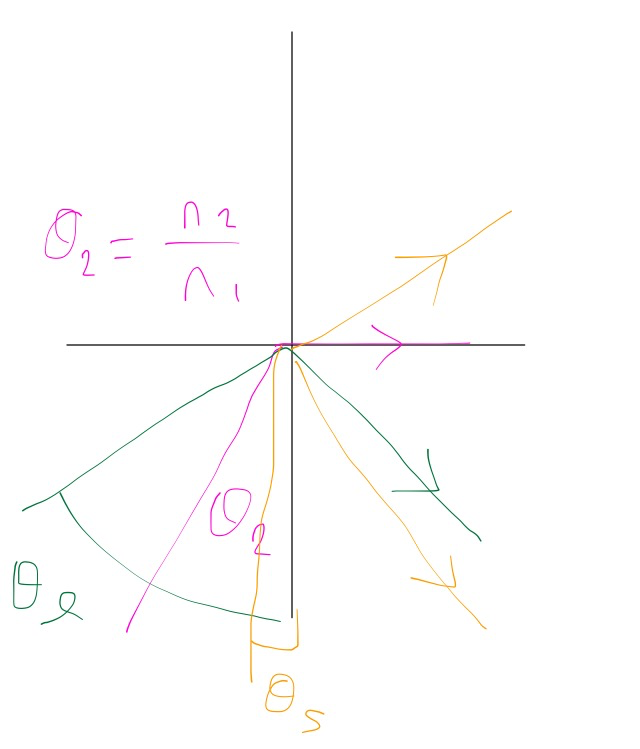
\includegraphics[scale=0.4]{q2}
							\end{center}
						\end{figure}
			  \end{enumerate}
		\item Unpolarized light is incident on water/air interface. At what angle should light be
			  incident to get 100\% polarization? Use the Brewster (polarization) angle.
			  	\begin{enumerate}
			  		\item C (incorrect, split): at $\theta_{p}$, reflected ray is polarized;
						  refracted ray remains unpolarized. Brewster's angle eqn
						% IMAGE Q3
  						\begin{figure}
							\caption{polarized reflected ray (Brewster's angle, Quiz 3)}
							\begin{center}
  								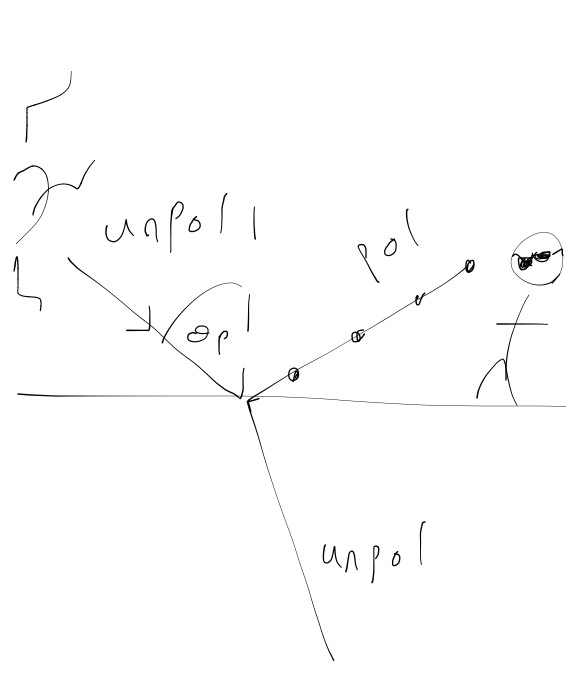
\includegraphics[scale=0.4]{q3}
							\end{center}
  						\end{figure}
			  	\end{enumerate}
	\end{enumerate}
	
	\section*{Mirrors}
	\begin{enumerate}
		\item object: every point of object emits rays in all directions
			\begin{enumerate}
				\item we only consider a few
			\end{enumerate}
		\item image: where the reflected rays converge (can be on either side of mirror)
	\end{enumerate}

\end{document}
